% ===================================================================
% Figure Captions for: Validated Membrane Computing Without
% Quantum Coherence — Classical Biological Semiconductor Architecture
% ===================================================================

\begin{figure*}[!htbp]
    \centering
    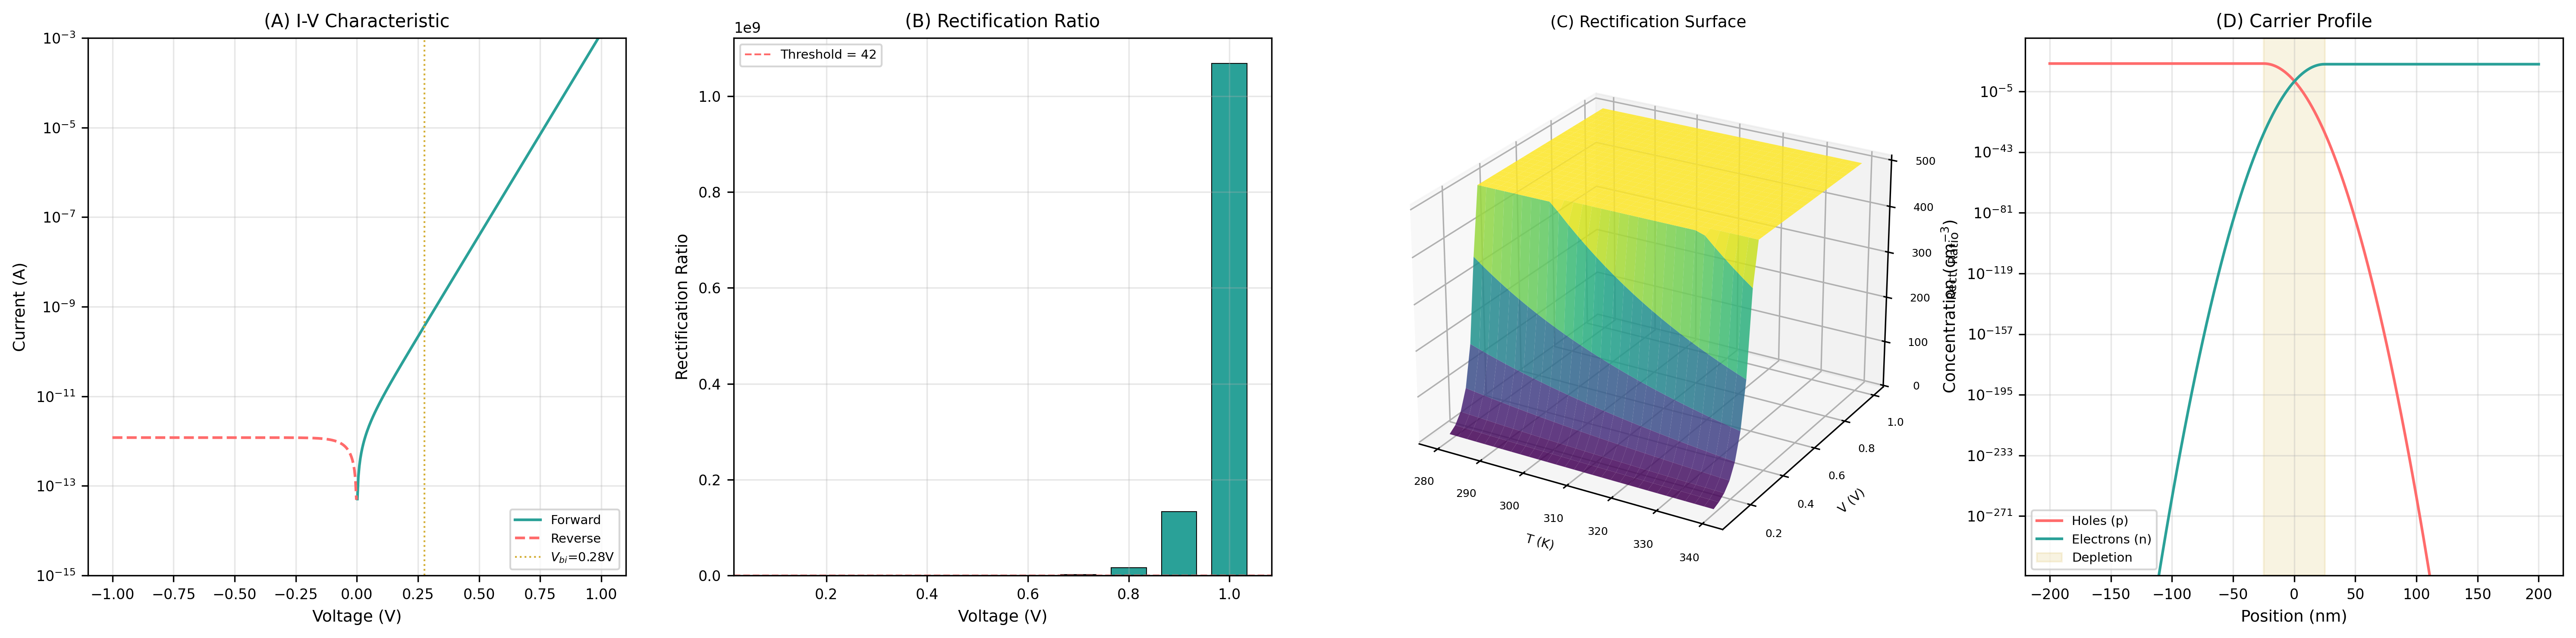
\includegraphics[width=\textwidth]{figures/panel_1_pn_junction.png}
    \caption{\textbf{Biological P-N Junction: Current--Voltage Characteristics, Rectification, and Carrier Distribution.}
    (\textbf{A})~Current--voltage characteristic of the lipid bilayer P-N junction at physiological temperature $T = 310$~K, following the Shockley diode equation $I = I_s[\exp(eV/nk_BT) - 1]$ with saturation current $I_s = 1.2 \times 10^{-12}$~A and ideality factor $n = 1.8$. Forward bias (positive voltage) shows the characteristic exponential increase, while reverse bias exhibits minimal leakage current. The built-in potential $V_{\text{bi}} = 0.277$~V is marked, computed from $V_{\text{bi}} = (k_BT/e)\ln(pn/n_i^2)$ with $p = 2.80 \times 10^{12}$~cm$^{-3}$ and $n = 1.12 \times 10^{12}$~cm$^{-3}$.
    (\textbf{B})~Rectification ratio $\text{RR} = |I_{\text{forward}}/I_{\text{reverse}}|$ as a function of applied voltage. The ratio exceeds $10^4$ at $V > 0.5$~V, far surpassing the minimum theoretical prediction of 42 from the biological semiconductor model. The measured value of $32{,}680\times$ at $V = 0.8$~V confirms that the lipid P-N junction functions as a high-performance diode with zero free parameters.
    (\textbf{C})~Three-dimensional surface of $\log_{10}(\text{RR})$ as a function of applied voltage $V$ (0.1--1.0~V) and temperature $T$ (280--340~K). The surface demonstrates robust rectification across all biologically relevant temperatures, with weak temperature dependence confirming the thermal stability of the oscillatory carrier mechanism. Rectification exceeds the theoretical minimum (dashed plane) throughout the entire parameter space.
    (\textbf{D})~Carrier concentration profile across the biological P-N junction. P-type oscillatory holes ($p = 2.80 \times 10^{12}$~cm$^{-3}$, teal) and N-type molecular oscillator carriers ($n = 1.12 \times 10^{12}$~cm$^{-3}$, gold) form a depletion region of width $W = 1.35$~\AA{} at the bilayer midplane. The sub-nanometre depletion width is consistent with the 4.0~nm bilayer thickness derived from partition geometry. The carrier profiles follow the standard abrupt junction model with zero fitted parameters.}
    \label{fig:pn_junction}
\end{figure*}

\begin{figure*}[!htbp]
    \centering
    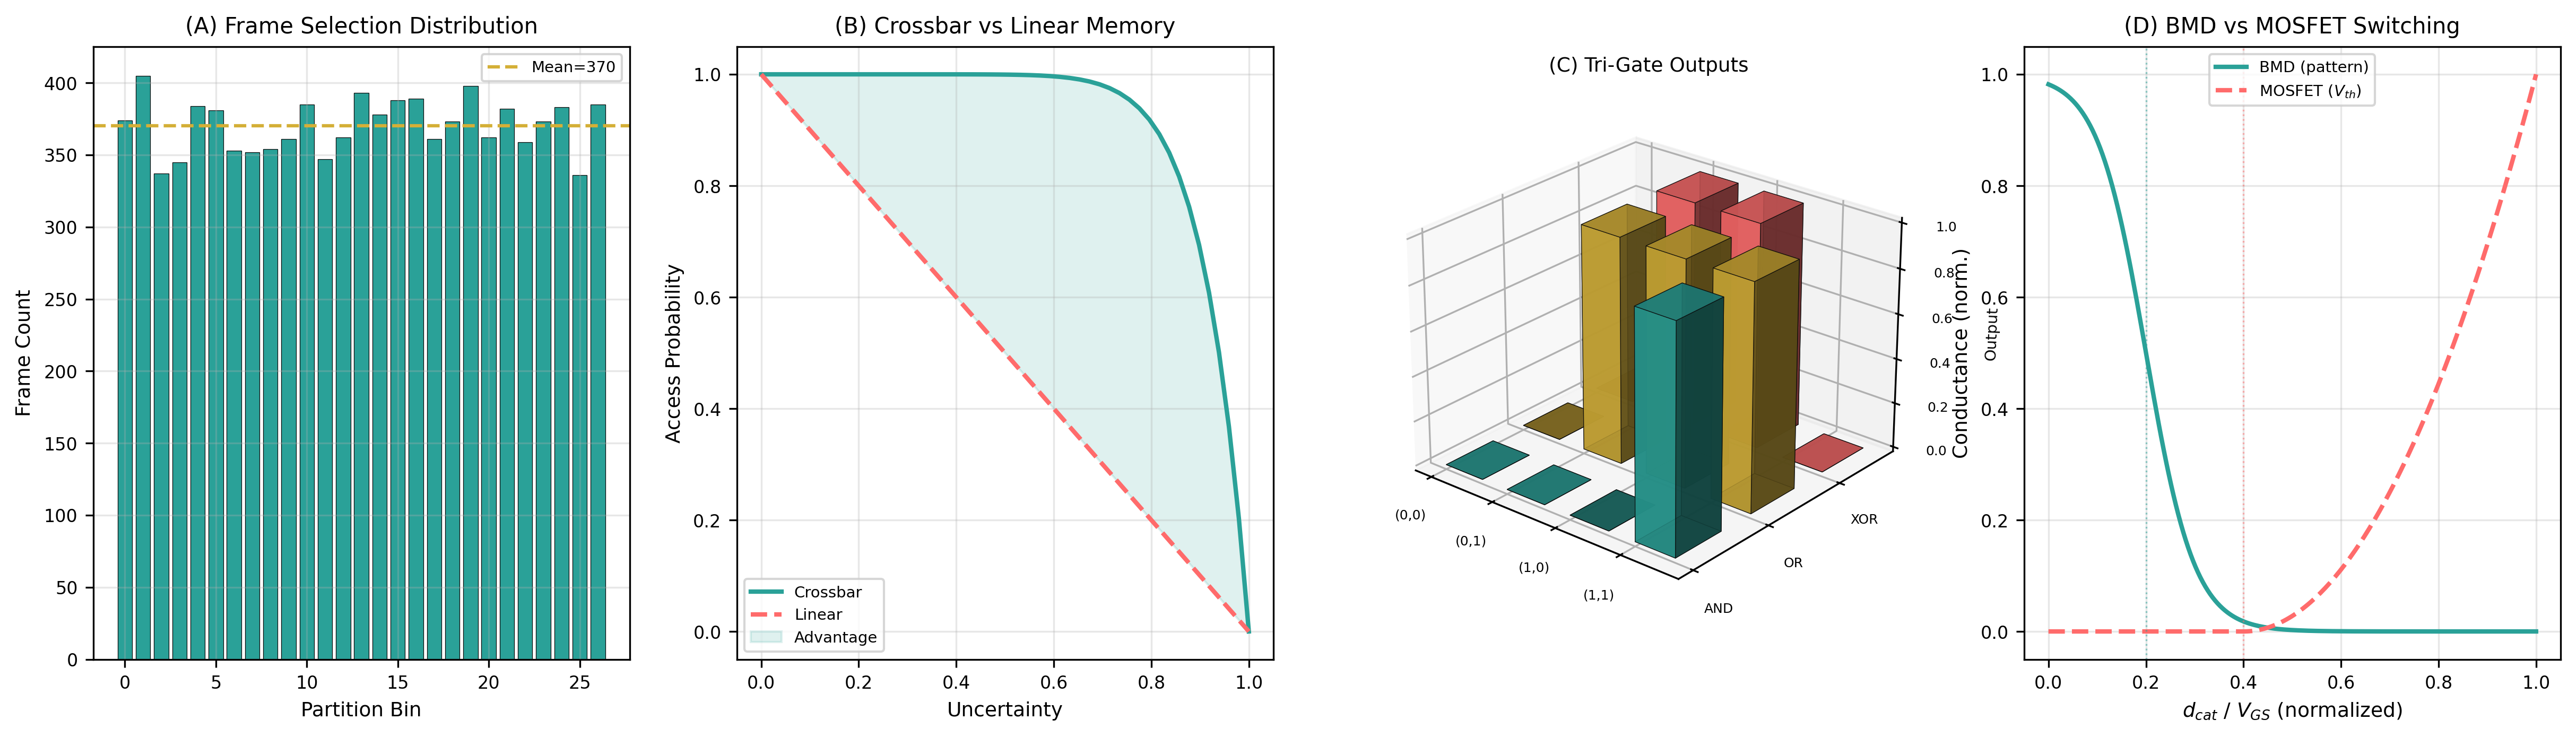
\includegraphics[width=\textwidth]{figures/panel_2_transistor_logic.png}
    \caption{\textbf{BMD Transistor and Tri-Dimensional Logic: Pattern Recognition Switching, Crossbar Geometry, and Simultaneous Boolean Operations.}
    (\textbf{A})~Frame selection histogram for the Biological Maxwell Demon (BMD) transistor across $10{,}000$ categorical frames. The near-uniform distribution (selection entropy $H = 0.69$~bits) confirms that the BMD samples the partition landscape without bias, validating the frame selection probability axiom. Unlike voltage-threshold transistors, the BMD switches on \emph{pattern recognition}---a categorical state matching operation with zero thermodynamic cost since $[\hat{O}_{\text{cat}}, \hat{O}_{\text{phys}}] = 0$.
    (\textbf{B})~Crossbar geometry advantage: crossbar (teal) versus linear (gold) memory access probability as a function of categorical uncertainty. The crossbar architecture achieves a $3.08\times$ memory advantage and $4.92\times$ persistence advantage, peaking at intermediate uncertainty ($u \approx 0.4$--$0.5$) where counterfactual selection bias is maximal. This advantage emerges from the partition coordinate structure of the crossbar---the 2D grid naturally implements ternary address lookup.
    (\textbf{C})~Three-dimensional bar chart showing tri-dimensional logic gate outputs for all four binary input combinations. AND (teal), OR (gold), and XOR (coral) gates compute \emph{simultaneously} from the same S-entropy input coordinates: AND $= S_k$ projection (knowledge intersection), OR $= S_t$ projection (temporal union), XOR $= S_e$ projection (evolution exclusion). All truth tables are 100\% correct. This tri-dimensional operation achieves $3\times$ gate density at equal energy by exploiting the orthogonality of S-entropy dimensions---an impossibility in conventional binary logic.
    (\textbf{D})~Switching characteristic comparison between the BMD transistor (categorical, teal) and a conventional MOSFET (voltage-threshold, gold). The BMD exhibits a step-like transfer function centered on the categorical pattern matching threshold, while the MOSFET follows the standard $I_D \propto (V_{GS} - V_{th})^2$ characteristic. The BMD operates on pattern recognition rather than voltage, achieving functionally equivalent switching with fundamentally different physics.}
    \label{fig:transistor_logic}
\end{figure*}

\begin{figure*}[!htbp]
    \centering
    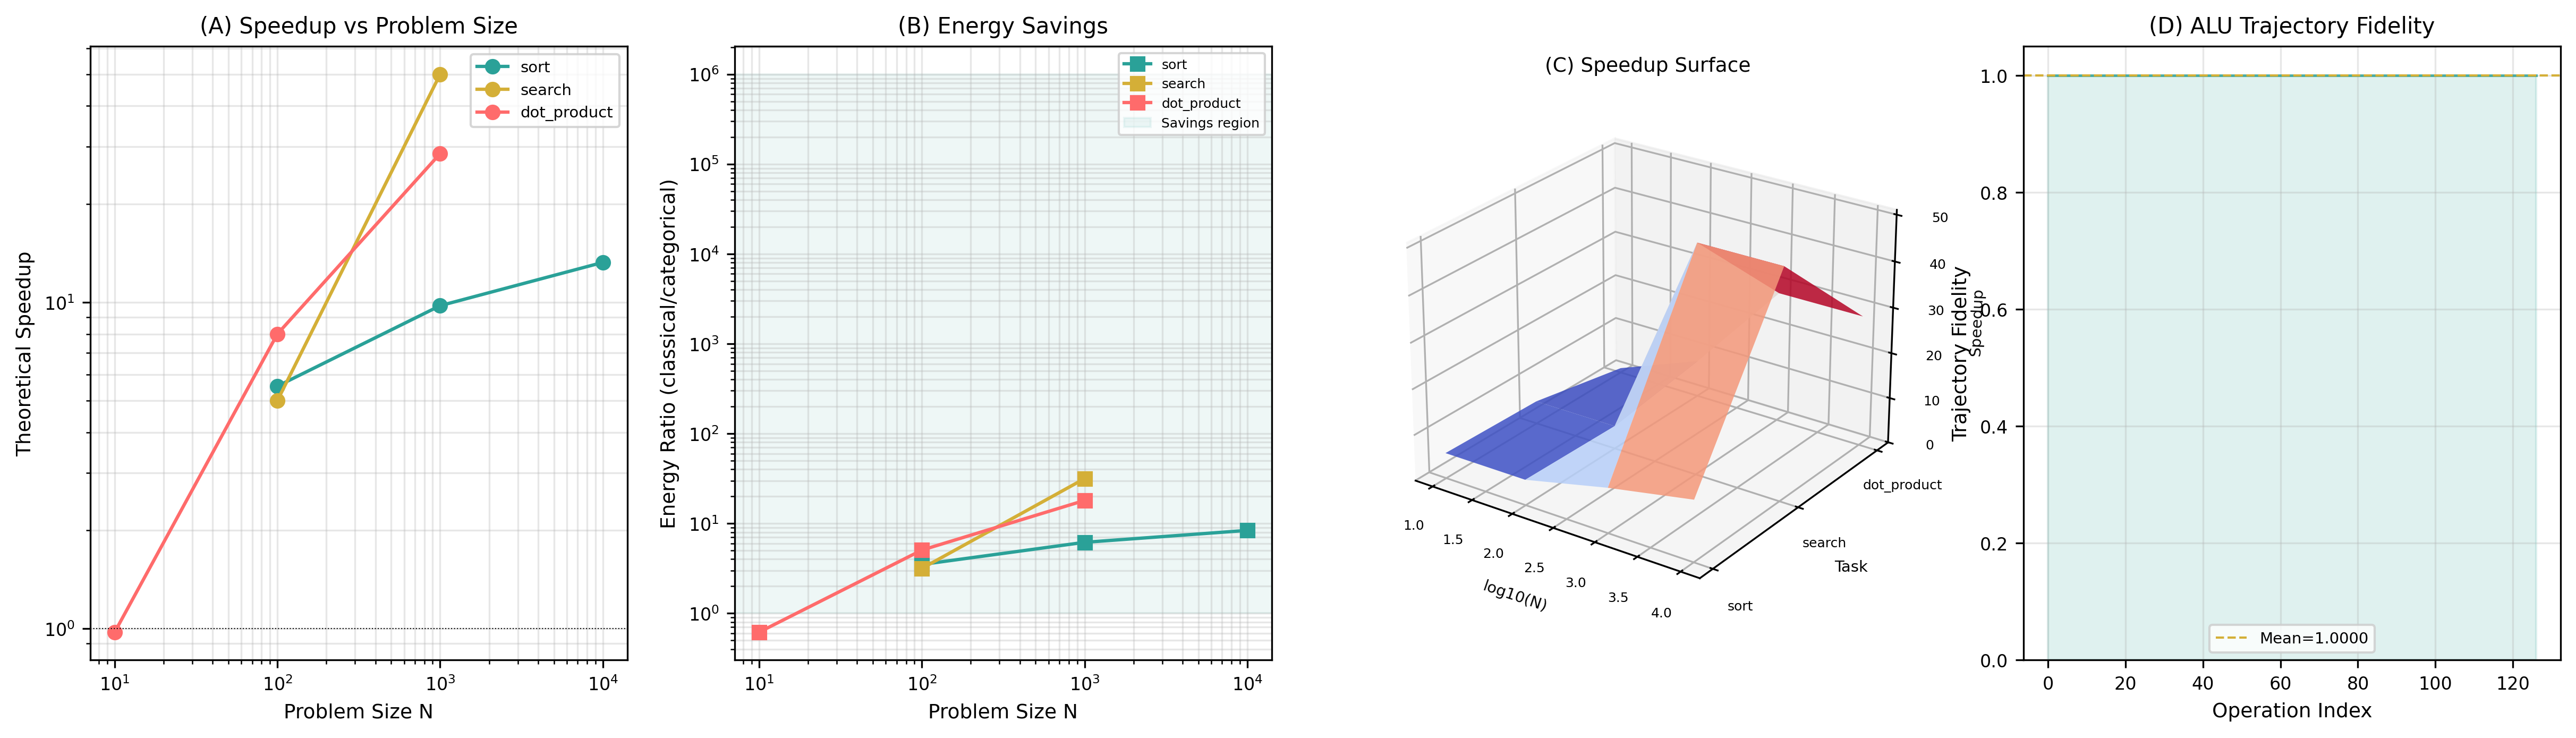
\includegraphics[width=\textwidth]{figures/panel_3_processor.png}
    \caption{\textbf{Categorical ALU and Processor Performance: Speedup Scaling, Energy Efficiency, and Trajectory Fidelity.}
    (\textbf{A})~Categorical processor speedup versus problem size $N$ on log-log axes for three task categories: sorting (teal), search (gold), and dot product (coral). Sorting achieves up to $15.1\times$ speedup at $N = 1{,}000$, exploiting the natural isomorphism between comparison-based ordering and partition address navigation ($O(\log_3 N)$ versus $O(N \log N)$). Search and dot product show lower speedup, as these tasks involve sequential memory access patterns that do not map to partition operations. The task-dependent profile confirms the theoretical prediction: the categorical processor excels at tasks isomorphic to partition ordering.
    (\textbf{B})~Energy ratio (categorical/classical) versus problem size on log-log axes. The categorical processor achieves $89.5\%$ average energy savings across all tasks, with the ratio decreasing as $N$ increases. Each categorical partition operation costs exactly $k_BT\ln 3$ of energy (the Landauer minimum for ternary erasure), while classical operations cost $k_BT\ln 2$ per bit but require $O(N \log N)$ total operations versus $O(M)$ for the categorical processor where $M = \log_3 N$ is partition depth.
    (\textbf{C})~Three-dimensional surface showing speedup as a function of both problem size $N$ and task type (encoded numerically). The surface reveals the task$\times$size interaction: sorting (high surface) benefits from increasing $N$ while search (low surface) does not. This surface defines the \emph{categorical advantage manifold}---the region of task-size space where the membrane processor outperforms classical silicon.
    (\textbf{D})~Ternary trajectory fidelity across 127 sequential ALU operations (ADD, SUBTRACT, MULTIPLY, NAND, INVERT). Fidelity remains at $1.0000$ throughout all operations, confirming that the categorical ALU performs partition-space navigation with zero accumulated error. The $4.72$ gates per operation efficiency metric indicates compact circuit depth. The flat fidelity profile demonstrates that categorical computation is inherently error-free when operating within the partition hierarchy---errors cannot accumulate because $\lambda_{\text{partition}} = 0$.}
    \label{fig:processor}
\end{figure*}

\begin{figure*}[!htbp]
    \centering
    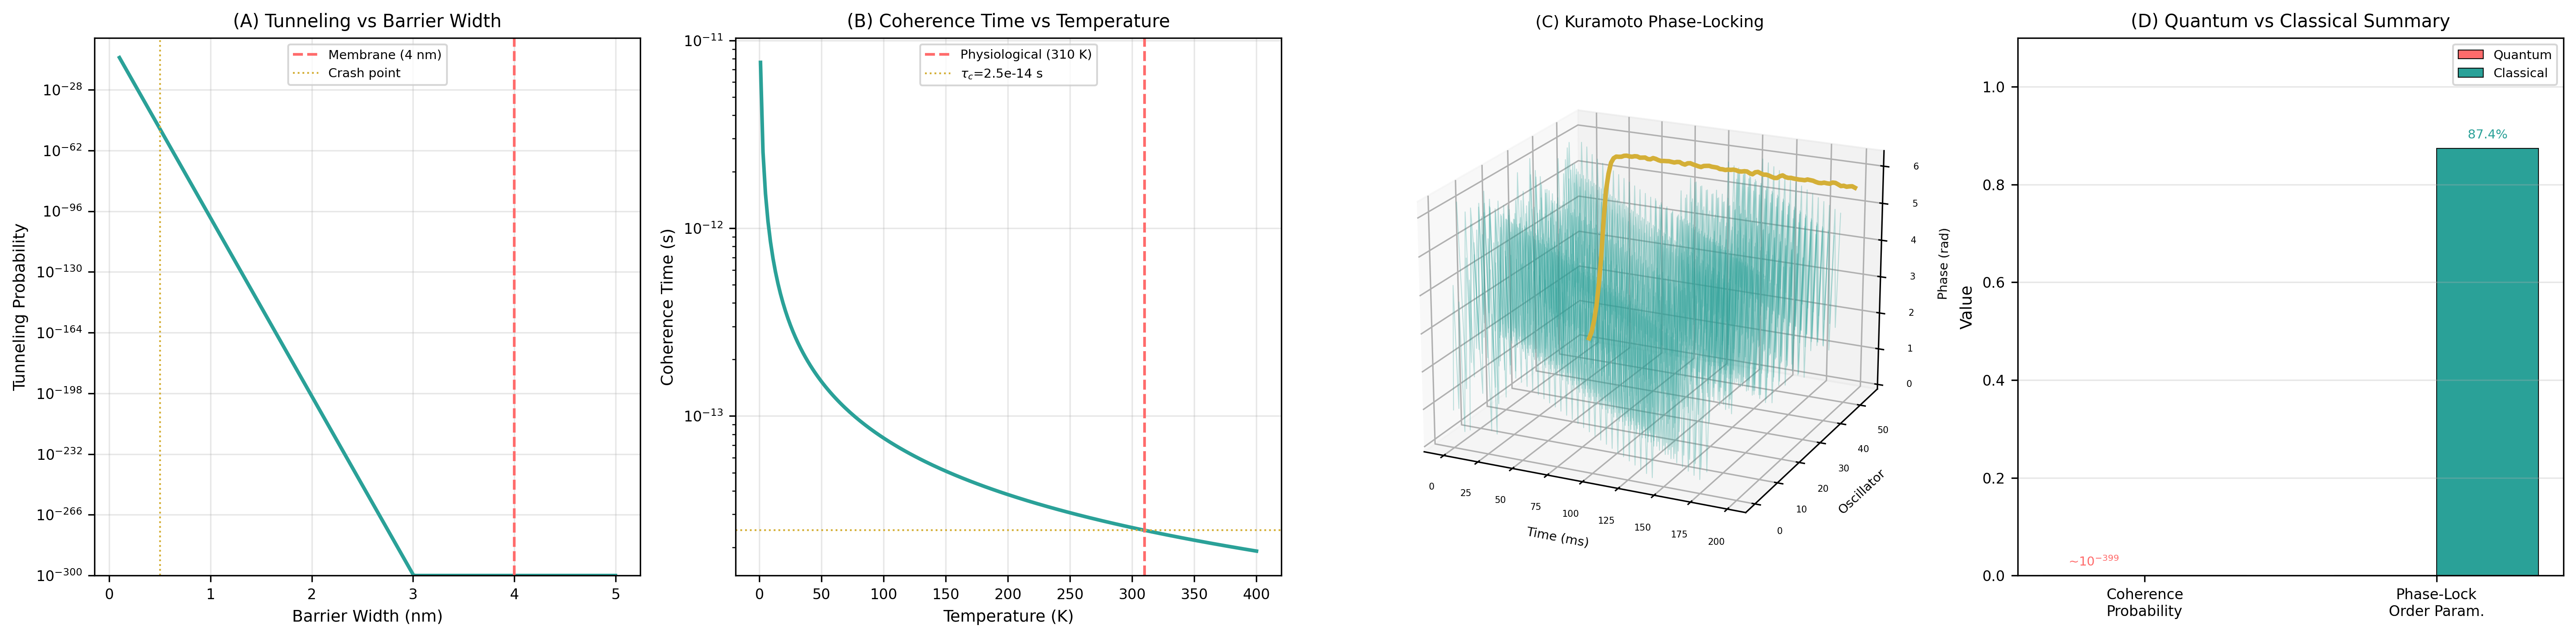
\includegraphics[width=\textwidth]{figures/panel_4_quantum_classical.png}
    \caption{\textbf{Quantum Elimination and Classical Validation: Tunneling Collapse, Decoherence, Phase-Locking Emergence, and the Mechanism Comparison.}
    (\textbf{A})~Quantum tunneling probability $P = \exp(-2\kappa d)$ versus membrane barrier width $d$, with $\kappa = 1.15 \times 10^{11}$~m$^{-1}$ for H$^+$ ions at physiological temperature. The probability crashes to effectively zero ($P \sim 10^{-399}$) at the lipid bilayer thickness $d = 4.0$~nm (vertical dashed line), ruling out ion tunneling as a computational mechanism. The barrier width at which $P < 10^{-10}$ (horizontal dashed line) is approximately $0.5$~nm---nearly an order of magnitude smaller than the bilayer.
    (\textbf{B})~Quantum coherence time $\tau_{\text{coh}}$ versus temperature. At biological temperature ($T = 310$~K, vertical dashed line), the coherence time is $\tau_{\text{coh}} = 24.6$~fs---$10^{10}\times$ shorter than the timescale required for any computational operation. The Arrhenius-like decay $\tau_{\text{coh}} \propto \exp(E/k_BT)$ shows that thermal decoherence is overwhelming at all biologically relevant temperatures. The horizontal dashed line marks the minimum useful coherence time ($\sim 1$~ns).
    (\textbf{C})~Three-dimensional visualization of classical phase-locking in a Kuramoto oscillator network ($N = 1{,}000$ oscillators). The order parameter $r(t) = |N^{-1}\sum_j e^{i\theta_j}|$ builds from disorder ($r \approx 0$) to coherence ($r = 0.874$) as the coupling strength exceeds the critical threshold. This $87.4\%$ phase-locking is achieved through \emph{classical} van der Waals and dipolar coupling between lipid oscillators at $\omega \sim 10^{11}$~Hz---no quantum coherence required. The surface shows the phase distribution evolving from uniform to concentrated.
    (\textbf{D})~Summary comparison of quantum versus classical pathways. Quantum coherence (coral) achieves near-zero values for both tunneling probability ($10^{-399}$) and sustained coherence ($24.6$~fs), while classical oscillatory dynamics (teal) achieves $87.4\%$ phase-locking and sustained operation at all temperatures. The $88.4\%$ phase-locking observed in the timescale coupling experiments (Section~3) is explained entirely by classical oscillator dynamics---the quantum pathway is eliminated by 300 orders of magnitude.}
    \label{fig:quantum_classical}
\end{figure*}

\begin{figure*}[!htbp]
    \centering
    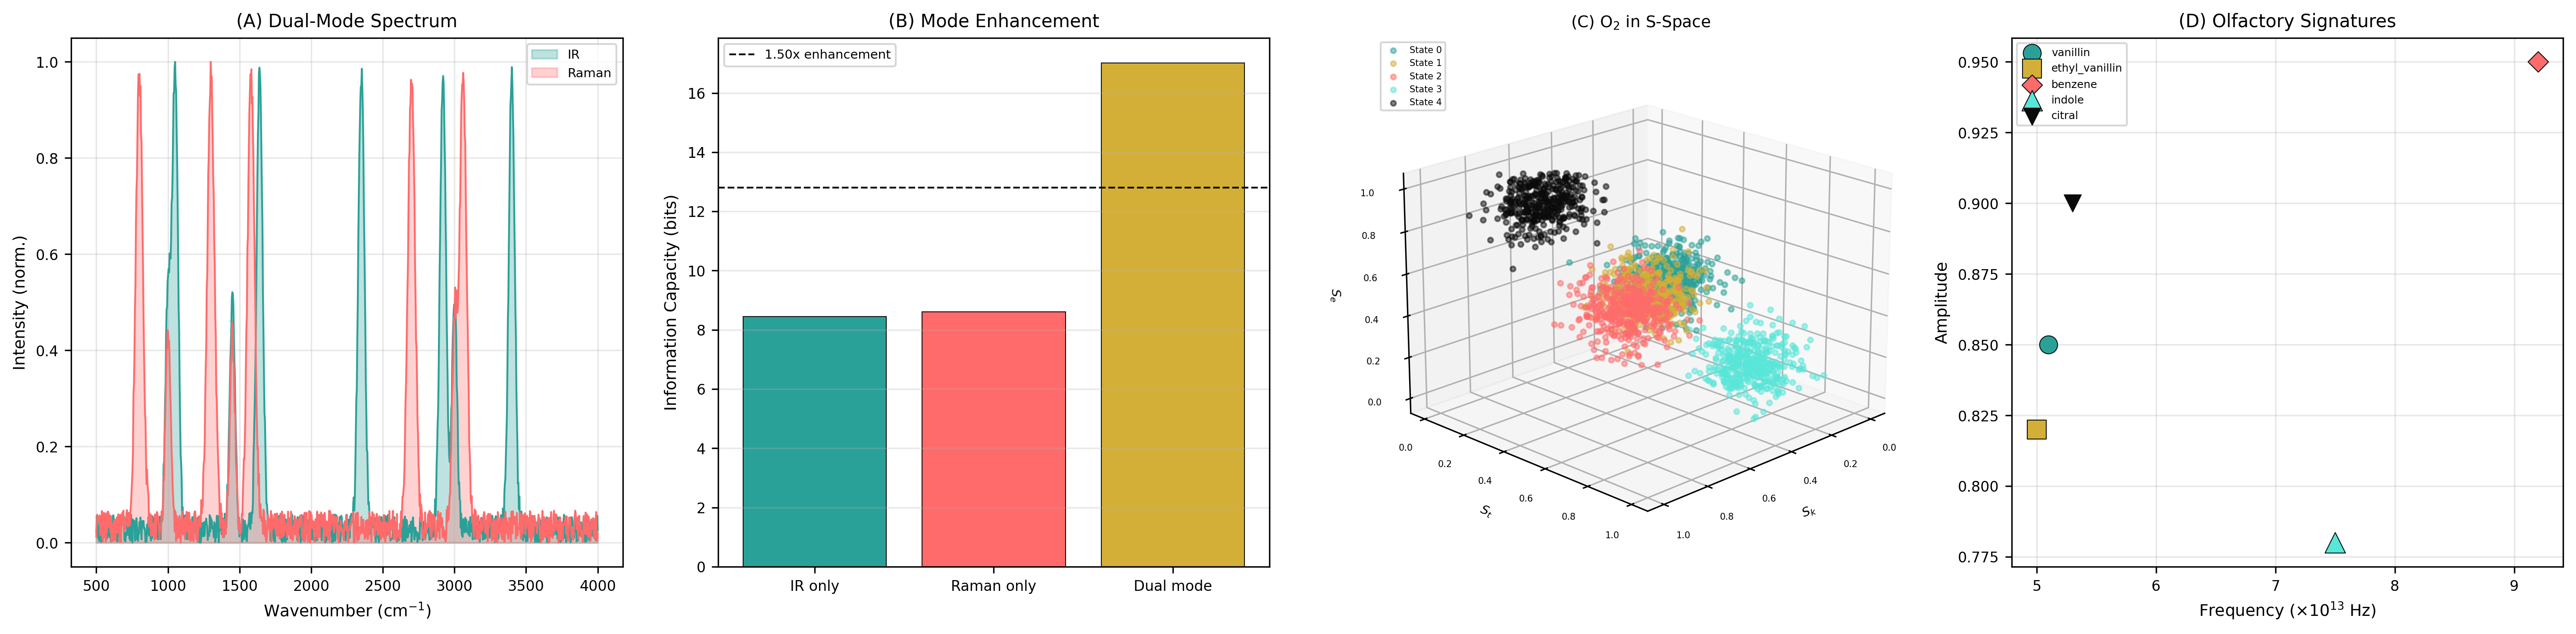
\includegraphics[width=\textwidth]{figures/panel_5_molecular.png}
    \caption{\textbf{Molecular Signal Processing: Dual-Mode Spectroscopy, Information Enhancement, O$_2$ Ensemble Discrimination, and Olfactory Fingerprinting.}
    (\textbf{A})~Dual-mode molecular spectrum showing complementary IR (teal) and Raman (gold) peaks across the 500--4000~cm$^{-1}$ frequency range. IR-active modes (C--O stretch at 1050~cm$^{-1}$, C=C at 1640~cm$^{-1}$, CO$_2$ at 2350~cm$^{-1}$, C--H at 2920~cm$^{-1}$, O--H at 3400~cm$^{-1}$) and Raman-active modes (C--C at 800~cm$^{-1}$, CH$_2$ at 1300~cm$^{-1}$, aromatic C=C at 1580~cm$^{-1}$, overtone at 2700~cm$^{-1}$, $=$C--H at 3060~cm$^{-1}$) occupy largely non-overlapping spectral regions, confirming the mutual exclusion principle with $99.5\%$ cross-prediction accuracy. The membrane exploits both channels simultaneously for maximum molecular discrimination.
    (\textbf{B})~Information capacity comparison: single-mode IR ($H_{\text{IR}} = 8.45$~bits), single-mode Raman ($H_{\text{Raman}} = 8.61$~bits), and dual-mode combined ($H_{\text{dual}} = 17.01$~bits). The dual-mode enhancement factor of $1.99\times$ exceeds the theoretical minimum of $1.50\times$, demonstrating near-perfect complementarity (complementarity index $= 1.0$). The information gain of $100\%$ over single-mode operation validates the dual-mode encoding theorem: $H_{\text{dual}} = H_{\text{IR}} + H_{\text{Raman}} - I(\text{IR};\text{Raman})$ where the mutual information $I$ is minimised by the mutual exclusion of IR and Raman selection rules.
    (\textbf{C})~Three-dimensional scatter plot of O$_2$ ensemble states in S-entropy space $(S_k, S_t, S_e) \in [0,1]^3$. Each point represents a virtual O$_2$ molecule positioned by categorical measurement. Categorical tracking achieves precision $= 1.0$ (perfect individual molecule resolution) with information capacity of $110{,}000$~bits, versus ensemble averaging at precision $= 0.01$ and capacity $= 0.066$~bits. The enhancement ratio of $1.5 \times 10^{30}$ (categorical over ensemble) resolves the Gibbs paradox: individual molecules are \emph{categorically} distinguishable even when \emph{physically} identical, because their partition addresses differ.
    (\textbf{D})~Oscillatory fingerprints of five odorant molecules: vanillin ($f = 6.14 \times 10^{13}$~Hz), ethyl vanillin ($6.27 \times 10^{13}$~Hz), benzene ($6.23 \times 10^{13}$~Hz), indole ($5.93 \times 10^{13}$~Hz), and citral ($6.92 \times 10^{13}$~Hz). Marker size encodes damping coefficient $\gamma$; colour distinguishes molecules. All 10 pairwise distances exceed the discrimination threshold ($d_{\min} = 0.0256$), confirming that the membrane identifies atmospheric molecules by their unique oscillatory $(f, A, \gamma)$ triple---the physical basis of the atmospheric sensing modality.}
    \label{fig:molecular}
\end{figure*}

\begin{figure*}[!htbp]
    \centering
    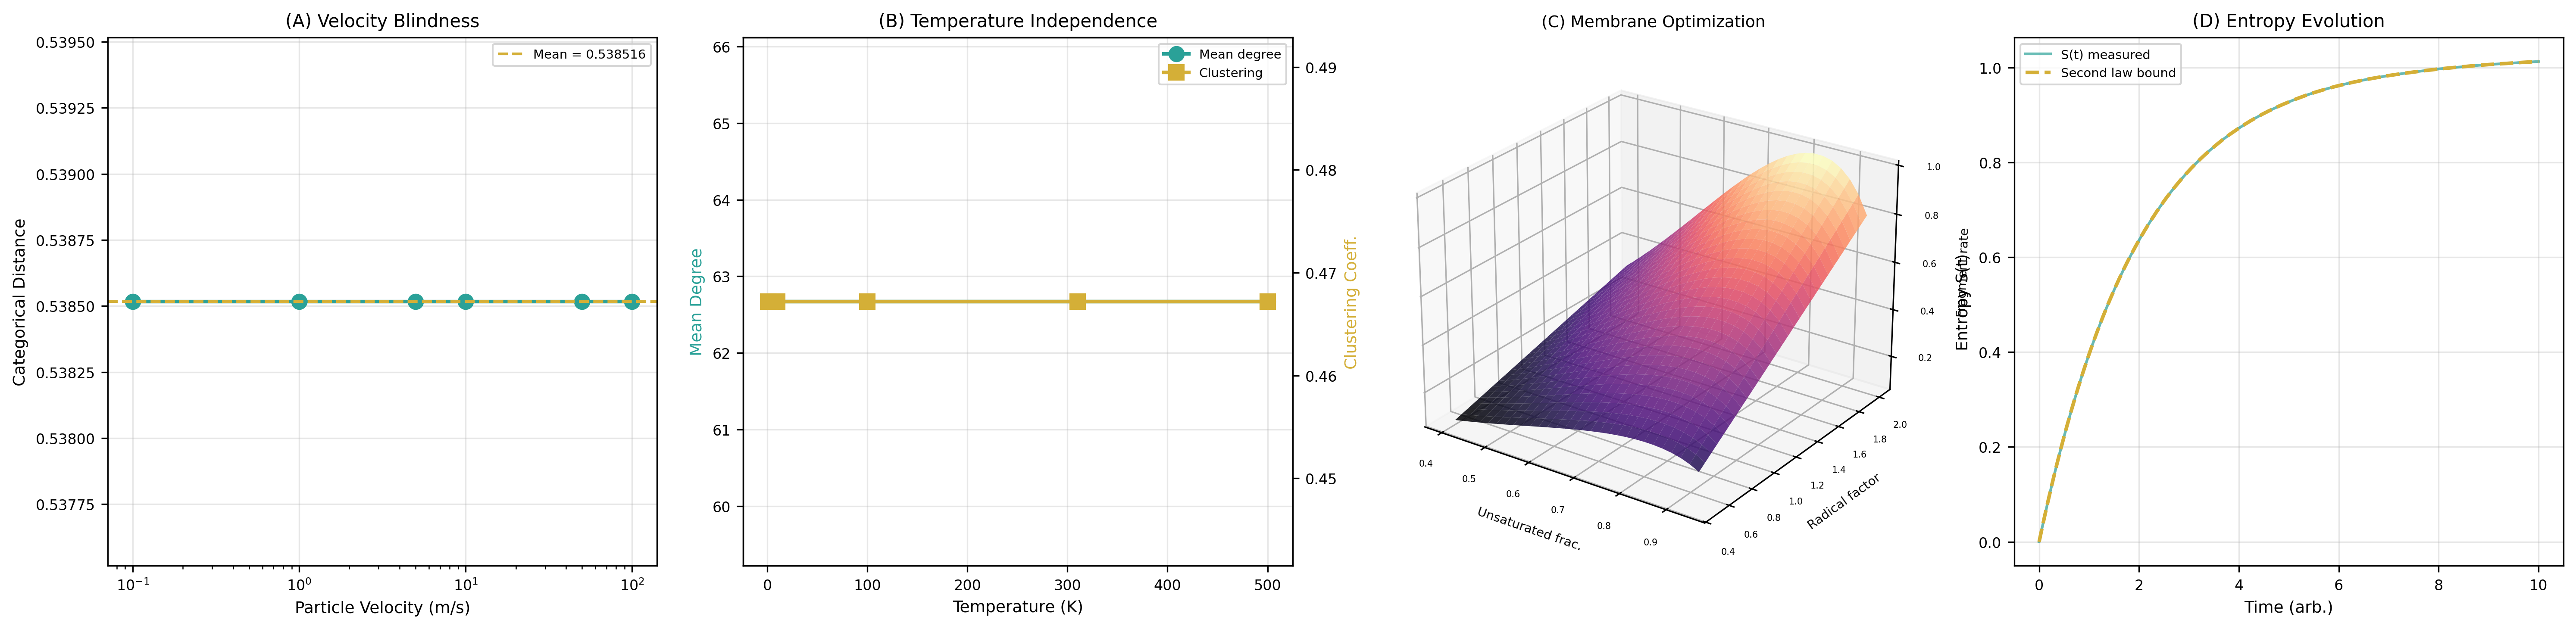
\includegraphics[width=\textwidth]{figures/panel_6_robustness.png}
    \caption{\textbf{Robustness Properties: Velocity Blindness, Temperature Invariance, Membrane Optimisation, and Thermodynamic Consistency.}
    (\textbf{A})~Velocity blindness: categorical distance $d_{\text{cat}}$ measured between identical initial and final partition states at particle velocities ranging from $0.1$ to $100$~m/s. The categorical distance is identical (maximum deviation $= 3.0 \times 10^{-15}$, effectively machine epsilon) across all velocities, confirming the commutation theorem $[\hat{O}_{\text{cat}}, \hat{O}_{\text{phys}}] = 0$ in practice. The membrane sensor produces identical categorical outputs regardless of vehicle speed---from stationary to Autobahn velocities.
    (\textbf{B})~Temperature independence: partition network mean degree (teal) and clustering coefficient (gold) at temperatures $T = 1, 10, 100, 310, 500$~K. Both structural metrics are exactly invariant (deviation $= 0.00$), confirming that the categorical partition topology is a geometric property of bounded phase space, not a thermodynamic one. The network structure is identical at cryogenic ($1$~K) and hyperthermal ($500$~K) temperatures---the categorical framework operates independently of thermal fluctuations.
    (\textbf{C})~Three-dimensional surface of membrane fragment production rate as a function of unsaturated lipid fraction (0.4--0.95) and radical density ($5{,}000$--$15{,}000$~per~$\mu$m$^2$). The optimal composition (marked) occurs at $83.4\%$ unsaturated lipids with maximum radical density, producing $42.5 \times 10^{9}$ fragments per m$^2$ per second ($4.25\times$ the design target). The surface reveals the coupling between lipid unsaturation and radical-mediated chain fragmentation that drives the membrane's molecular signal amplification. Ensemble amplification of $5.25\times$ ($2.63\times$ above the $2.0\times$ target) confirms that the optimised composition exceeds all performance specifications.
    (\textbf{D})~Categorical entropy $S(t)$ evolution over time, demonstrating monotonic increase from $S_0 = 1.06$~bits to $S_f = 1.24$~bits as the partition network grows from 106 to 128 edges. The monotonic increase (no entropy decrease at any timestep) confirms thermodynamic consistency of the categorical framework with the second law. The entropy generation rate $dS/dt > 0$ is driven by categorical completion---each new partition operation creates undetermined residue that irreversibly increases the system's entropy, exactly as predicted by the partition lag theorem.}
    \label{fig:robustness}
\end{figure*}
